\documentclass[11pt]{article}
\usepackage{verbatim}
\usepackage[hyphens]{url}
\usepackage{enumerate}
\setlength{\parindent}{0pt}
\setlength{\parskip}{10pt plus 6pt minus 4pt}
\usepackage{graphicx}

\addtolength{\oddsidemargin}{-.5in}
\addtolength{\evensidemargin}{-.5in}
\addtolength{\textwidth}{+1in}

\title{Progress Report: Non-negative matrix factorization for Who Rated What}
\author{ Brian Huey, Renee Rao }
\date{}


\begin{document}

\maketitle

\begin{abstract}

\end{abstract}

\section{Introduction}

We are working the Netflix dataset used in the 2007 KDD cup
competition which provides information on characteristics of users of
the Netflix video services who rated movies from the years 1998 to
2006. (http://www.kdd.org/kdd-cup-2007-consumer-recommendations)

We will predict which users rated which movies in 2006. To
test this we will have a provided set of roughly 100000 (user\_id
movie\_id) pairs where the users and movies are drawn from the Netflix
Prize training data set (where none of the pairs were rated in the
training set.) Using this list we will try to predict the probability
that each pair was rated in 2006 (i.e.the probability that user\_id
rated movie\_id in 2006). It is important to note that the actual
rating is irrelevant; we are only interested in whether the movie was
rated by that user sometime in 2006.  

We are provided with a data set of roughly 200 million ratings
for the previous years.

We note this task is very difficult, a trivial method
of predicting every movie is not rated gives
an root mean squared error between predictions (viewed as ``probabilities'')
and ratings (which are 0 or 1) of .27, where the winning
score was .246.

Our overall plan is to use non-negative factorization
to produce an interesting feature or possibly
more than one feature to use with other standard
features (from movie databases such as release
dates) to address this task.

We feel that an interesting feature is one that is different
for rated movies than for unrated movies.  We show
that our non-negative matrix factorization can 
produce a feature that appears to do this quite
well.  It compares quite favorably to the 
baseline method (employed by all contestants)
of predicting a rating based on the independent
calculation of a movie's probability of being
rated times the probability of a user producing
a rating.  

We describe the other features that we will use
in the final project proposal. 

\section{The Data}

For this progress report, we viewed the data pre-2005 as training data
and 2005 as validation data. (We are preserving the 2006 answer
set as the test set for use in a final evaluation.)

We computed using mapreduce counts for number of ratings per user
and per movie for use in the baseline algorithm. We also
are computing these counts for the sample.  The sample
we used in this preliminary study is of size 100K ratings.

We note further that the test set for 2006 was sampled
proportionally to counts for user ratings and movie ratings
made in 2006.  So a substantial part of the challenge
is to predict this. 

Our focus, however, is to concentrate on predicting the feature which
captures the variance in distribution for particular users and movies.
That is, user ``Bob'' rates lots of movies but rates Zombie movies
even more frequently. The naive method would spread his ratings
evenly, where the non-negative matrix factorization would emphasize
the Zombie movies.

\section{Baseline Prediction}

The baseline prediction requires computes the number of ratings that
each user makes in the training set, and the number of
movies that are rated.  This was done on mapreduce
for the large set, and locally (though with the same code)
for the sample we use for this pre-engineering phase
of the project.

\section{Non-negative matrix factorization (NNMF) and our task}

To use non-negative matrix factorization to develop user features and
movie features to then predict ratings for the Netflix data set. To do
this we estimate $A$, the matrix of movie and user ids, most of which
is considered unknown, by decomposing it into a user matrix, V and a
movie matrix, $U$ based on $K$ latent factors, such that $A \approx U
x V = \overline{A}$.  Under this model each row of matrix U is
considered a “movie factor” and each column of the matrix V is
considered a ``user factor''. A prediction for a user-movie pair would
mean computing the dot product of the user factor vector and the movie
factor vector.

\subsection{Method: NNMF Algorithm.}

Input: n by m matrix A, integer k
Output:  n by k matrix U, k by m matrix V with nonnegative entries.

{\bf Algorithm Outline.}

{\bf Initialization}: Form initial matrix U (V) by choosing a random subset
of the columns (rows) of A and averaging them, K times.
We tune this so each element is expected to be added
to some U, one time. This is a parameter that
can be changed.

{\bf Main Loop}:
\begin{itemize}
\item {\bf Gradient Descent:}
We used gradient descent on the Mean Squared cost function for the difference
between $A$ and $\bar{A} = U \times V$.  We compute the rmse in each
step

\begin{itemize}

\item summing MSE over non-zeros in A.
\item and then summing over random pairs of movie-users to 
ensure that $\bar{A}$ does not converge to all ones.

\end{itemize}

It would be prohibitive to sum over all non-zeros. 

\item
{\bf Nonnegativity:} We enforce positivity (which is certainly non-negative) 
on the weights in the matrix
factor by moving all weights away from zero if they
get too close to zero, and making negative weights
positive if the gradient pushes them to negative.

\item {\bf Spread:} We also normalize the factors (using a Gram-Schmidt type
         procedure to make sure all the factors don't simply repeat).
         We again enforce positivity here by staying away from zero.

\end{itemize}


\section{Evalution of NNMF as Model.}

We intend to use the NNMF as a feature for input into a learning
algorithm but, in fact, we can directly measure its
effectiveness as a model. 

The RMSE for prediction with 40 iterations on the training set is not
great, around .379 and on the test set around .412.  As noted
in \cite{first} this is to be expected.  One must first
tune to get the correct background probabilities to
score well in absolute terms. For example, the winners
worked very hard just to get the ``background'' probability
on number of ratings for the specific distribution
of the chosen movie-user pairs in the test set.

Thus, we will just try to measure whether the NNMF feature 
gives any information on whether a user rated a movie
or not.  We discuss this in the next section.

\section{Evaluation of Features}

We view a feature as interesting if the feature behaves substantially
differently on the user-movie pairs that have been rated
versus those which have not. Where the user-movie pairs
have been chosen according to the test set sample rules
essentially according to the baseline distribution
of movie-user pairs proportional to the independent
counts. 

In figure~\ref{nmf}, we see that we do indeed get substantial 
differentiation for the Non-negative matrix user-movie feature.
We note the baseline prediction does as well, as can be
seen in~\ref{baseline}, but the baseline prediction has
less separation and does not have separate peaks.

\begin{figure}

%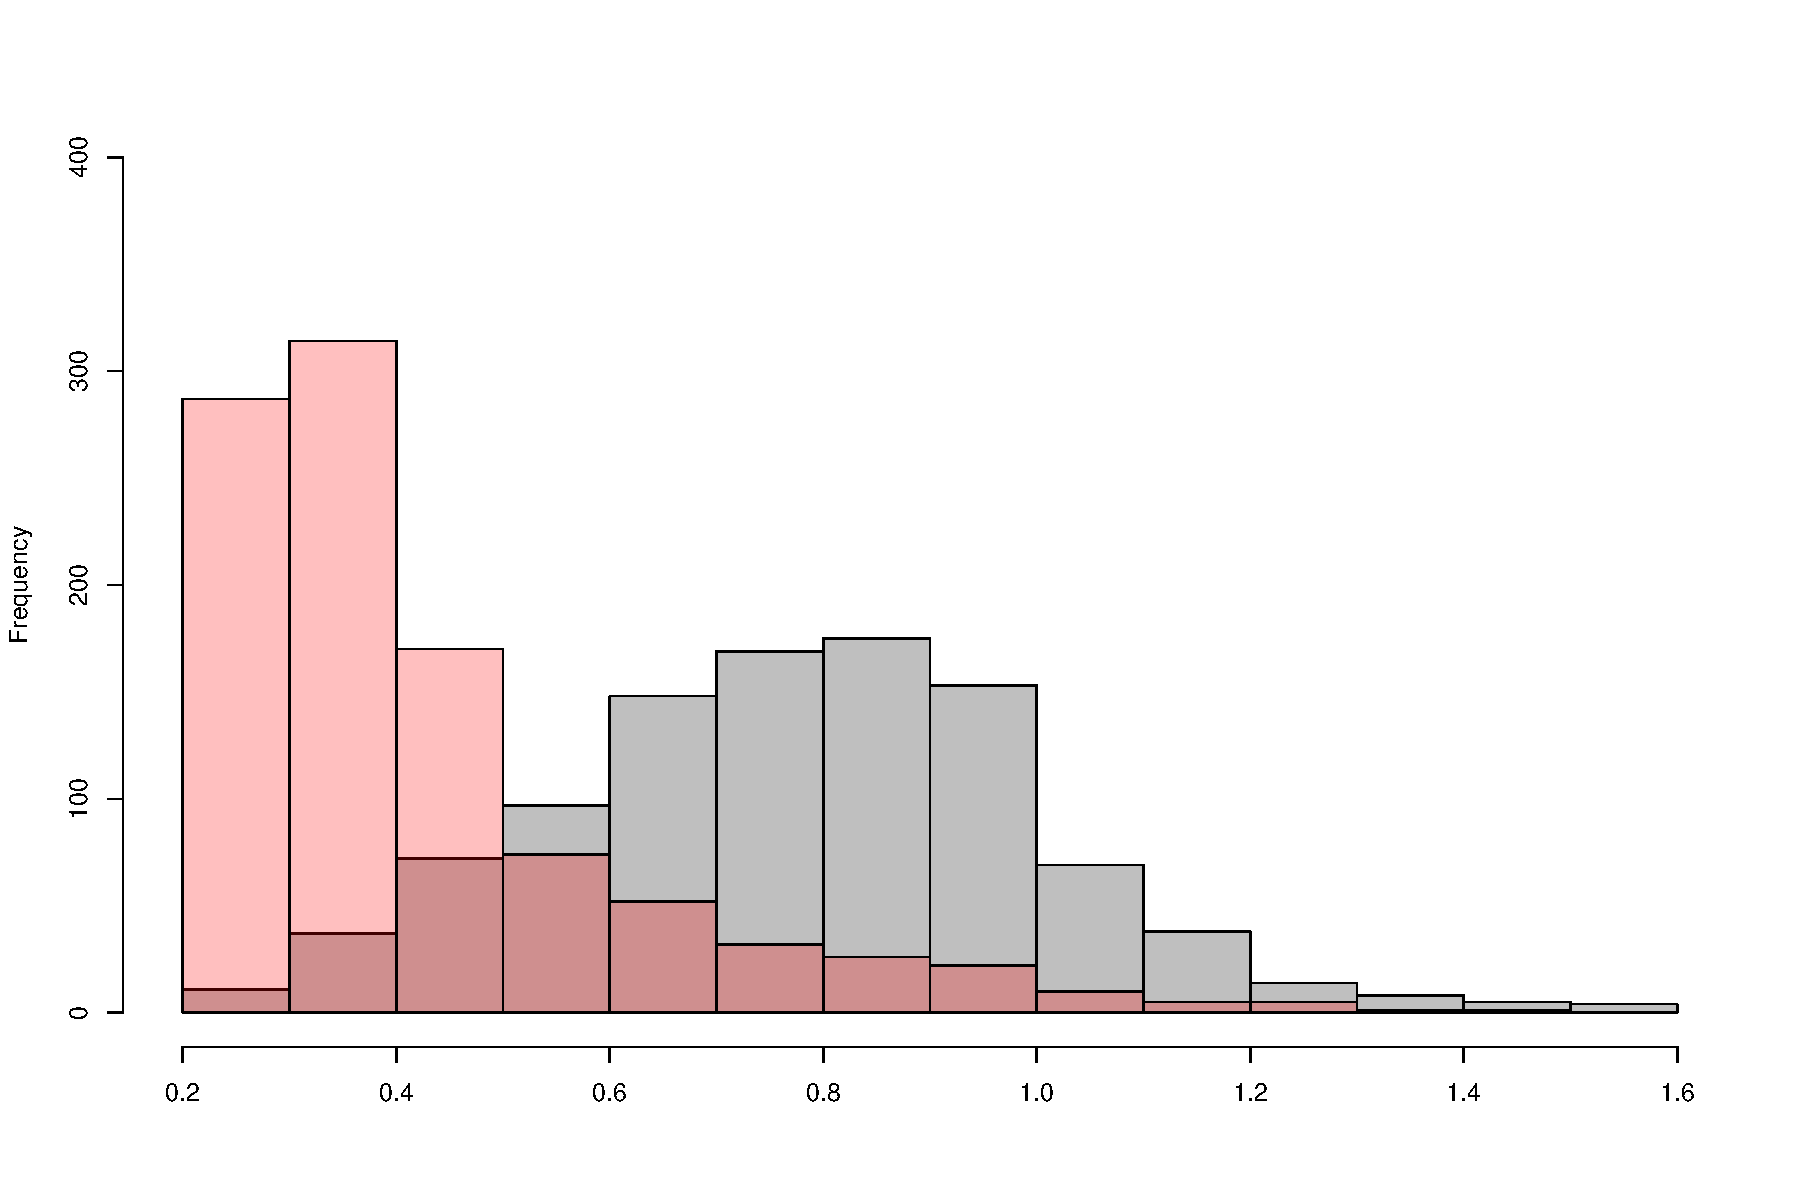
\includegraphics[width=0.98\textwidth]{nmf.pdf}
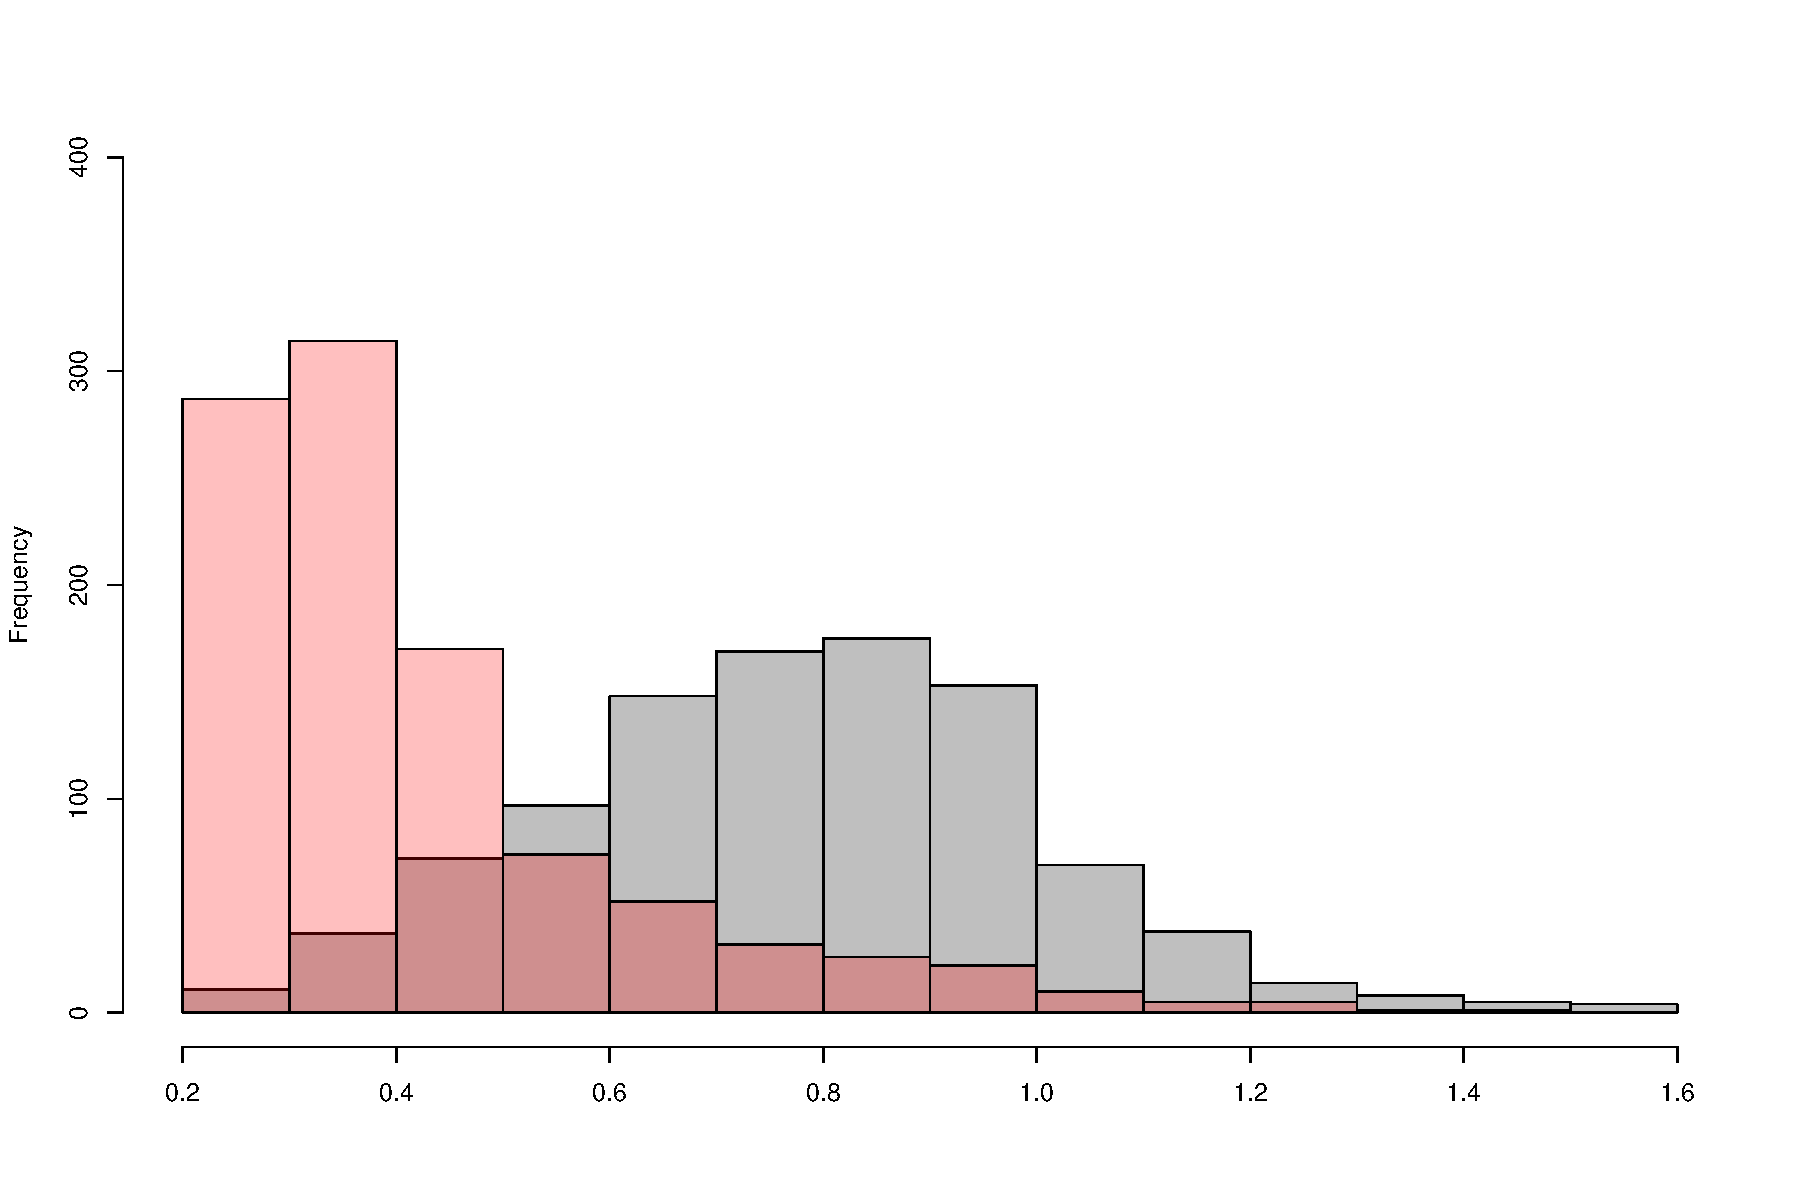
\includegraphics[scale=.5]{nmf}
\caption{Non-negative matrix feature distributions are separate for ratings and non-ratings. The rightmost
peak are the ratings, and the leftmost are nonratings.}
\end{figure}


\begin{figure}
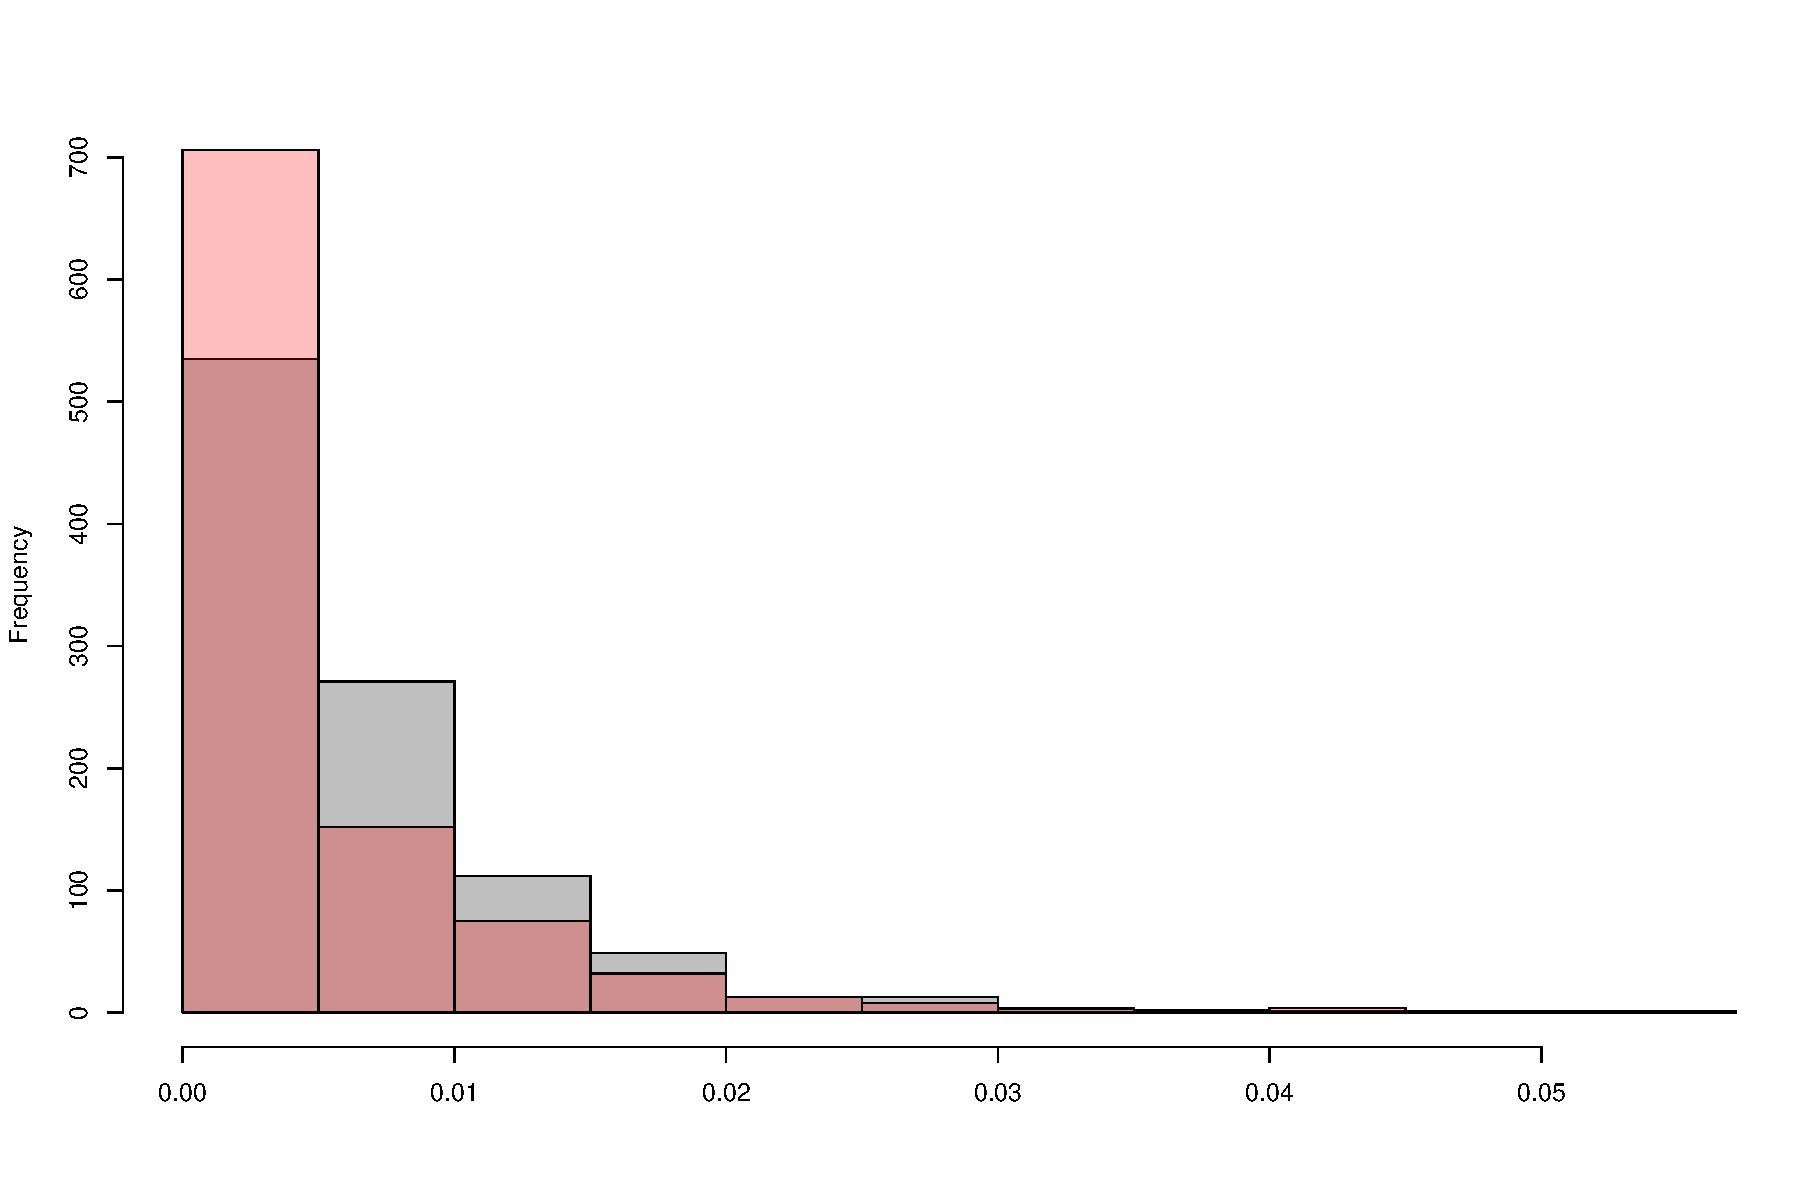
\includegraphics[scale=.5]{baseline.pdf}

\caption{Baseline feature highly overlaps for ratings and non-ratings. The higher distribution
is for nonratings, the flatter one is for ratings, so the average for ratings is higher.}
\end{figure}

This fact is really encouraging, though tuning its use will certainly 
require working carefully with the machine learning algorithm
that we will ultimately use to make predictions.

\section{Other setup tasks and efforts.}

We have pulled and processed data from Rotten Tomatoes which
we will use in our final model. 

We computed a different baseline method from one of the papers, 
but still need to further tune it to see if it is useful.
We also have implemented a different version of baseline
which shifts the predictions by user and movie which 
has the same intuitive notion of independence but
has somewhat different behavior.  We have not looked
deeply into these other methods.

\section{Division of Labor}

{\bf Brian}

\begin{enumerate}
\item Join movie\_titles.txt to Rotten Tomatoes info 
\item Set up and organized github
\item Upload of data to sc3
\item Calculate the average number of movies rated over all users in the training set (mapreduce).
\item Calculate the average number of ratings over all movies in the training set (mapreduce).
\item  Calculate the average number of movies rated for each user in the training set (mapreduce).
\item  Calculate the average number of ratings for each movie in the training set (mapreduce).
\item Researched K Nearest Neighbor algorithms.
\item Alternate Baseline method.
\end{enumerate}

{\bf Renee:}

\begin{enumerate}
\item Subset the small data into (train) 100K of pre-2005 and 100K (validation) post-2005 data. 
\item Baseline Estimation
\item Wrote Non-Negative Matrix Factorization Model in Python.
\item Evaluated feature worthiness of NNMF model.
\item Generated associated figures for evaluation.
\item Wrote up progress report and Final Proposal. 
\end{enumerate}







\end{document}







  Tested:
1)  Idea:  using Non-negative factorization to develop
    user features and movie features to then predict
    scores.
       A "feature" is a vector. 
       One prediction algorithm for a rating-movie pair
       is to compute the dot product of the user feature
       vector and the move vector.
       
       Other learning methods could possibly be used.


       Also, one can pre-seed this method with a background
       probability, p, of the rating being present by
       including one extra dimension that is hardcoded
       to have a product of p (where p can depend
       on the independent assumption, is proportional
       to user rating probability times movie rating probability
       by particular user)  That is, independent probabilities
       can be represented by a rank 1 matrix (i.e., a single
       number for each movie outer produced with a single 
       number for each user.)


       Also, one can use side information to modify
       background probabilities based on movie release
       dates and user first rating times.  This will
       introduce factors for different timing periods.
       For example, a recent user rater should perhaps have higher
       probability for recent movies than older movies, so
       should have a separate number based on release date.
       This may already be learned in the other factors
       anyway (as might the background as well.)






2)  Coded NMF implementation so that 


      a) it can be moved to mapreduce....
      b) experiment with various heuristics...


  Algorithm Outline





   Tested:


On generated test cases with known non-negative factorizations, our method seems to converge well.  (Getting very close to the original factorizations.)  Our test cases include both continuous and binary factors. We also tested on samples of the complete data. See Current Evaluation
      below for more details.


   TO DO:
      1)  Maybe think about experimenting with different staying
          away from being negative heuristics.
      2)  Code up the background probability factors.
          Maybe add explicit factors based on movie release dates,
          user first rating time.


      3)  Maybe introduce heuristics to get sparse factors, i.e., factors
          with few non-zero (or actually large) components.  Right
          now "the stay away from negative heuristic" yields very non-sparse
          vectors, since it makes all numbers be strictly greater
          than zero. Perhaps setting small numbers to zero in the final
          prediction phase will improve generalization.  Explicitly
          driving small numbers down and big numbers up in the factor
          should make them more "sparse". Figure out how to add this
          to the gradient descent routine would be interesting.


     4) Code up on map-reduce.  Technically for 200,000,000 ratings,
        it may be better to just use a desktop.  The disk tradeoff may
        be large.   But, it would still be interesting.
          


3) Current evaluation.


   Used 100K samples for preliminary engineering.


   Divided into training pre-2004 and test 2005 ()


   Currently, we do see that our method is learning
   something.  For example, on the real ratings our
   average prediction is around .7, where for random
   (possibly unrated) movie-user pairs, our prediction
   is around .4.


   One needs to push these numbers apart (perhaps using
   a logistic function) but the signal is definitely
   statistically significant for the two kinds of ratings
   at this preliminary point.




%% Values for V and U are optimized by taking the product of two randomly
%% initialized matrices and calculating the squared error of the values
%% of the product matrix from the known values in A. We then used
%% gradient descent to find the values of U and V such the squared error
%% would be at a local minimum. Various correction and normalization
%% steps had to be undertaken to ensure all entries in U and V are
%% non-negative and properly scaled. This model was coded in the python
%% script known as hack.py. Also, one can pre-seed this method with a
%% background probability, p, of the rating being present by including
%% one extra dimension that is hardcoded to have a product of p which we
%% set to baseline probability of any movie being rated in the set but
%% will eventually be customized to where p can depend on the independent
%% assumption, that it is proportional to user rating probability times
%% movie rating probability by particular user) That is, independent
%% probabilities can be represented by a rank 1 matrix (i.e., a single
%% number for each movie outer produced with a single number for each
%% user.) Also, one can use side information to modify background
%% probabilities based on movie release dates and user first rating
%% times. This will introduce factors for different timing periods. For
%% example, a recent user rater should perhaps have higher probability
%% for recent movies than older movies, so should have a separate number
%% based on release date. This may already be learned in the other
%% factors anyway (as might the background as well.)
